\documentclass[runningheads]{llncs}

\usepackage{listings}
\usepackage[colorlinks]{hyperref}

\usepackage[x11names]{xcolor}

\usepackage[ruled]{algorithm2e}
\usepackage{amsmath,amsfonts}

\usepackage[utf8]{inputenc}

\lstset{
    basicstyle=\fontsize{9}{9}\selectfont\ttfamily,
    keywordstyle={[1]\color{Blue4}\bfseries}, % keywords style
    keywordstyle={[2]\color{Pink4}}, % type style
    keywordstyle={[3]\color{OrangeRed3}}, % function style
    literate =
        {=>}{{=>}}2
        {/=}{{/=}}2,
    commentstyle=\itshape\color{gray}
}

\lstdefinestyle{C}{
    language = C,
    classoffset = 1,
    morekeywords = {Socket, IpAddr, uint_t, uint16_t, error_t},
    classoffset = 2,
    morekeywords = {socketOpen, socketConnect},
    classoffset = 0
}

\lstdefinestyle{Spark}{
    language = Ada,
    classoffset = 1,
    morekeywords = {Socket_Struct, Socket, Not_Null_Socket, Socket_Type, Socket_Prot, IpAddr, Error_T, Port},
    classoffset = 2,
    morekeywords = {Socket_Open, Socket_Connect, Socket_Send},
    classoffset = 7,
    morekeywords = {Pre, Post},
    keywordstyle = \bfseries,
    classoffset = 0,
}

\let\Spark\lstinline

\let\state\textsf
\let\flag\textsf

\usepackage{tikz}
\usetikzlibrary{decorations.pathreplacing, patterns}
\usetikzlibrary{calc, backgrounds}

\usepackage{subcaption}

\title{Verification of a TCP/IP stack}

\author{Guillaume Cluzel\inst{1,2} \and
        Yannick Moy\inst{1} \and
        Cl\'ement Zeller\inst{3}}


        \institute{Adacore \and
        \'Ecole Normale Sup\'erieure de Lyon \and
        Oryx Embedded}


\begin{document}

\authorrunning{G. Cluzel et al.} %, Y. Moy and C. Zeller}

\maketitle

\begin{abstract}
    The abstract should briefly summarize the contents of the paper in
    150--250 words.

    \keywords{First keyword  \and Second keyword \and Another keyword.}
\end{abstract}

\section{Introduction}

    In the development of the Internet, the TCP protocol that has a very special place.
    Initially described by the ``fathers of the Internet'' Vincent Cerf and Bob Kahn, the TCP protocol was standardized in 1981 by RFC 793~\cite{rfc793}.
    Since this date, TCP has been widely used on the Internet as the underlying protocol for application layers such as HTTP,
    FTP or TLS. TCP is based on the underlying IP protocol which is itself
    based on a link layer such as Ethernet. This stacking of protocols is referred to as the TCP/IP stack.

    Given the importance of the TCP protocol in network communications, some researchers have attempted to formalize the protocol to either prove key properties~\cite{smith1996formal}
    or even to fully prove the correctness of an implementation against a complete specification~\cite{ridge2008rigorous}.
    This latter implementation was performed in the HOL proof assistant, and while the authors note that it would be possible in theory to extract an implementation in Haskell from
    this work, this has not been adopted in practice.
    The formalization of TCP specification and verification of a TCP implementation face two difficulties:
    RFC 793 is written in English, leaving many parts underspecified; the TCP protocol is inherently concurrent which makes it complex to specify and verify.
    As a result, there is currently no formally verified implementation for TCP that is usable in industry.

    Other communication protocols have been formalized in recent years, leading to a formally verified implementation.
    The most prominent project in this area is the Everest project~\cite{bhargavan2017everest}, which led to a formally verified implementation in F* of TLS called miTLS~\cite{bhargavan2013implementing}.
    Note that miTLS still relies on an untrusted implementation of TCP, and thus could benefit from the results of our work.
    The approach taken in project Everest was to reimplement the formalized protocols completely in F*, a research programming language targeted at formal program verification.
    This approach is often difficult to adopt in industry, as codebases are evolved incrementally rather than replaced, both for economical and practical reasons.

    Our approach in this work has been to incrementally evolve an existing TCP/IP stack in C by replacing parts of the code with formally verified code in SPARK.
    The stack chosen, CycloneTCP\footnote{\url{https://www.oryx-embedded.com/products/CycloneTCP.html}}, is targeted at embedded processors with no Operating System.
    In Section~\ref{sec:TCP} we describe the TCP protocol, in particular the state machine that governs the behavior of a connection.
    In Section~\ref{sec:spec} we present specificities of the specification technique that we used, and in Section~\ref{sec:verif} we explain how we formalized and implemented in SPARK the TCP user functions and the underlying socket API.
    In Section~\ref{sec:results} we present the results of our work, in particular bugs that have been found and eliminated thanks to our approach, before we conclude.

\section{TCP protocol and CycloneTCP library}
\label{sec:TCP}

\subsection{TCP protocol}

The TCP protocol is one of the most used protocol on the Internet.
It is connection-oriented in the sense that a connection requires to be
established between the two processes that exchange data. The protocol is
governed by a state machine described in figure~\ref{Fig:statemachine}.
The whole description of the protocol can be found in RFC~793~\cite{rfc793}.
Its implementation is rather free and lots of choices are left to the programmer.
However, the implementation must ensure some properties to be able to communicate
with other TCPs.
We present here the main elements that are useful for our verification.


\begin{figure}[t]
    {\centering\scalebox{.55}{
    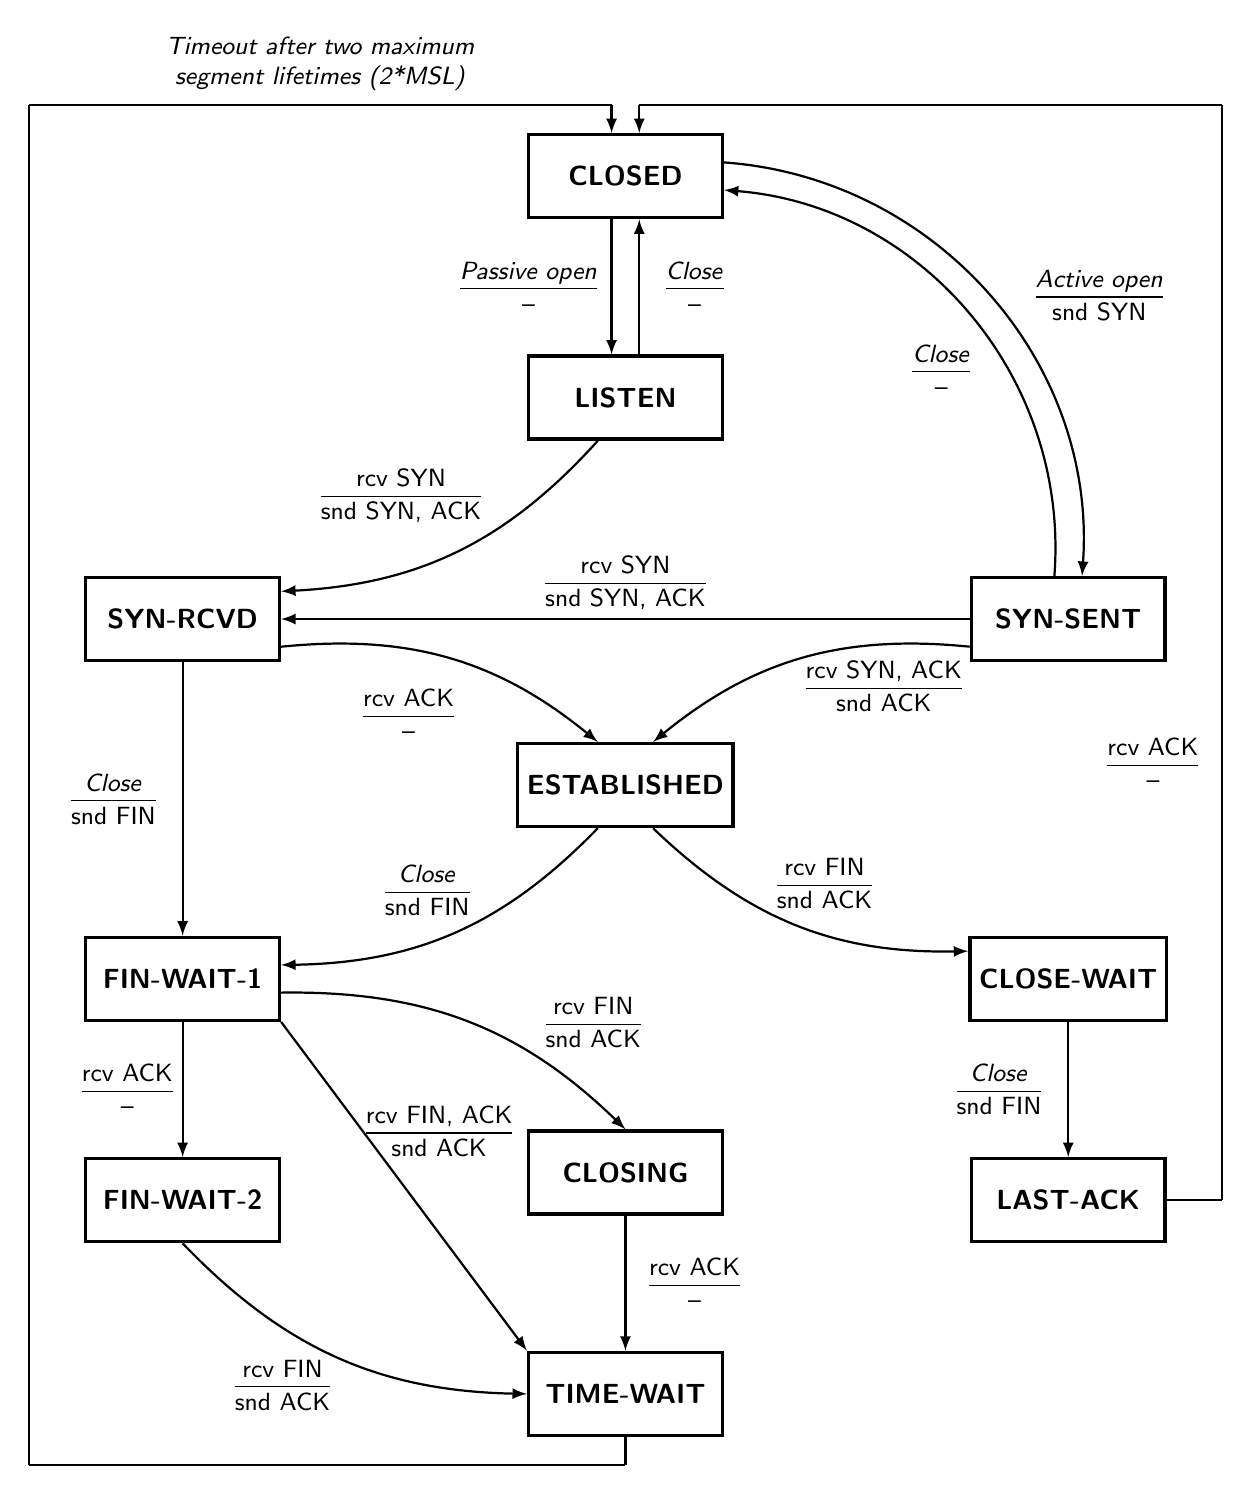
\begin{tikzpicture}[>=latex]
        \def\tfrac#1#2{\ensuremath{\displaystyle\frac{\text{\small#1}}{\text{\small#2}}}}
        %
        % Styles for states, and state edges
        %
        \tikzstyle{state} = [draw, very thick, fill=white, rectangle, minimum height=3em, minimum width=7em, node distance=8em, font={\sffamily\bfseries}]
        \tikzstyle{stateEdgePortion} = [black,thick];
        \tikzstyle{stateEdge} = [stateEdgePortion,->];
        \tikzstyle{edgeLabel} = [pos=0.5, text centered, font={\sffamily\small}];

        %
        % Position States
        %
        \node[state, name=closedStart] {CLOSED};
        \node[state, name=listen, below of=closedStart] {LISTEN};
        \node[state, name=synSent, below of=listen, right of=listen, xshift=8em] {SYN-SENT};
        \node[state, name=synRcvd, below of=listen, left of=listen, xshift=-8em] {SYN-RCVD};
        \node[state, name=established, below of=listen, node distance=14em] {ESTABLISHED};
        \node[state, name=finWait1, below of=established, left of=established, node distance=7em, xshift=-9em] {FIN-WAIT-1};
        \node[state, name=finWait2, below of=finWait1] {FIN-WAIT-2};
        \node[state, name=closeWait, below of=established, right of=established, node distance=7em, xshift=9em] {CLOSE-WAIT};
        \node[state, name=closing, below of=established, node distance=14em] {CLOSING};
        \node[state, name=lastAck, below of=closeWait] {LAST-ACK};
        \node[state, name=timeWait, below of=closing] {TIME-WAIT};

        %
        % Connect States via edges
        %
        \draw ($(closedStart.south) + (-.5em,0)$)
        edge[stateEdge] node[edgeLabel, xshift=-3em]{\tfrac{\emph{Passive open}}{--}}
        ($(listen.north) + (-.5em,0)$);
        \draw ($(listen.north) + (.5em,0)$)
        edge[stateEdge] node[edgeLabel, xshift=2em]{\tfrac{\emph{Close}}{--}}
        ($(closedStart.south) + (.5em,0)$);

        \draw ($(listen.south) + (-1em,0)$)
        edge[stateEdge, bend left=22.5] node[edgeLabel, xshift=-2em, yshift=2em]{\tfrac{rcv SYN}{snd SYN, ACK}}
        ($(synRcvd.east) + (0,1em)$);

        % \draw ($(synRcvd.north) + (.5em,0)$)
        % edge[stateEdge, bend left=45] node[edgeLabel,xshift=-4em]{\emph{Timeout}/RST}
        % ($(closedStart.west) + (0,-.5em)$);

        \draw ($(synSent.north) + (-.5em,0)$)
        edge[stateEdge, bend right=45] node[edgeLabel,xshift=-1em, yshift=-2em]{\tfrac{\emph{Close}}{--}}
        ($(closedStart.east) + (0,-.5em)$);
        \draw ($(closedStart.east) + (0,.5em)$)
        edge[stateEdge, bend left=45] node[edgeLabel,xshift=4em]{\tfrac{\emph{Active open}}{snd SYN}}
        ($(synSent.north) + (.5em,0)$);

        \draw (synSent.west)
        edge[stateEdge] node[edgeLabel, yshift=1.3em]{\tfrac{rcv SYN}{snd SYN, ACK}}
        (synRcvd.east);
        \draw (synRcvd)
        edge[stateEdge] node[edgeLabel, xshift=-2.5em]{\tfrac{\emph{Close}}{snd FIN}}
        (finWait1);

        \draw ($(synRcvd.east) + (0,-1em)$)
        edge[stateEdge, bend left=22.5] node[edgeLabel, xshift=-1.5em, yshift=-2em]{\tfrac{rcv ACK}{--}}
        ($(established.north) + (-1em,0)$);
        \draw ($(synSent.west) + (0,-1em)$)
        edge[stateEdge, bend right=22.5] node[edgeLabel, xshift=3em, yshift=-1em]{\tfrac{rcv SYN, ACK}{snd ACK}}
        ($(established.north) + (1em,0)$);

        \draw ($(established.south) + (-1em,0)$)
        edge[stateEdge, bend left=22.5] node[edgeLabel, xshift=-1em, yshift=1.5em]{\tfrac{\emph{Close}}{snd FIN}}
        ($(finWait1.east) + (0,.5em)$);
        \draw ($(established.south) + (1em,0)$)
        edge[stateEdge, bend right=22.5] node[edgeLabel, xshift=1em, yshift=1.5em]{\tfrac{rcv FIN}{snd ACK}}
        ($(closeWait.west) + (0,1em)$);

        \draw (finWait1.south)
        edge[stateEdge] node[edgeLabel, xshift=-2em]{\tfrac{rcv ACK}{--}}
        (finWait2.north);
        \draw ($(finWait1.east) + (0,-.5em)$)
        edge[stateEdge, bend left=22.5] node[edgeLabel, yshift=0em, xshift=4.5em]{\tfrac{rcv FIN}{snd ACK}}
        (closing.north);
        \draw (finWait1.south east)
        edge[stateEdge] node[edgeLabel, xshift=0em, yshift=2em, text width=3em]{\tfrac{rcv FIN, ACK}{snd ACK}}
        (timeWait.north west);

        \draw (finWait2.south)
        edge[stateEdge, bend right=22.5] node[edgeLabel, xshift=-2em, yshift=-1em]{\tfrac{rcv FIN}{snd ACK}}
        (timeWait.west);

        \draw (closing)
        edge[stateEdge] node[edgeLabel, xshift=2.5em]{\tfrac{rcv ACK}{--}}
        (timeWait);

        \draw (closeWait)
        edge[stateEdge] node[edgeLabel,xshift=-2.5em]{\tfrac{\emph{Close}}{snd FIN}}
        (lastAck);

        %
        % Connect lastAck to closed is slightly more complicated
        % no direct line-of-sight, so we need to take the scenic route
        %
        \coordinate (lastAck2ClosedA) at ($(lastAck.east) + (2em,0)$);
        \coordinate (lastAck2ClosedB) at ($(closedStart.north -| lastAck.east) + (2em,1em)$);
        \coordinate (lastAck2ClosedC) at ($(closedStart.north) + (0.5em,1em)$);
        \draw (lastAck.east) edge[stateEdgePortion] (lastAck2ClosedA);
        \draw (lastAck2ClosedA) edge[stateEdgePortion] node[edgeLabel,xshift=-2.5em, yshift=-4em]{\tfrac{rcv ACK}{--}} (lastAck2ClosedB);
        \draw (lastAck2ClosedB) edge[stateEdgePortion] (lastAck2ClosedC);
        \draw (lastAck2ClosedC) edge[stateEdge] ($(closedStart.north) + (0.5em,0)$);

        %
        % likewise for timeWait to closed
        %
        \coordinate (timeWait2ClosedA) at ($(timeWait.south) + (0,-1em)$);
        \coordinate (timeWait2ClosedB) at ($(timeWait.south -| finWait2.west) + (-2em,-1em)$);
        \coordinate (timeWait2ClosedC) at ($(closedStart.north -| finWait2.west) + (-2em,1em)$);
        \coordinate (timeWait2ClosedD) at ($(closedStart.north) + (-0.5em,1em)$);
        \draw (timeWait.south) edge[stateEdgePortion] (timeWait2ClosedA);
        \draw (timeWait2ClosedA) edge[stateEdgePortion] (timeWait2ClosedB);
        \draw (timeWait2ClosedB) edge[stateEdgePortion] (timeWait2ClosedC);
        \draw (timeWait2ClosedC) edge[stateEdgePortion]
        node[edgeLabel, text width=12.25em, yshift=1.5em]{\emph{Timeout after two maximum segment lifetimes (2*MSL)}}
        (timeWait2ClosedD);
        \draw (timeWait2ClosedD) edge[stateEdge] ($(closedStart.north) + (-0.5em,0)$);

        % draw dotted lines around passive and active closes
        % \begin{pgfonlayer}{background}
        %     \draw [join=round,black,dotted] ($(closeWait.north west) + (-1em, -1em)$) rectangle ($(lastAck.south east) + (1em, 1em)$);
        %     \draw [join=round,black,dotted] ($(finWait1.north west) + (-1em, -1em)$) rectangle ($(timeWait.south east) + (1em, 1em)$);
        % \end{pgfonlayer}

    \end{tikzpicture}}\par}
    \caption{TCP state machine.}
    \label{Fig:statemachine}
\end{figure}


\subsubsection{States}

In this automaton, the states represent the state of the connection. \state{CLOSED}
stands for a closed connection. Both states \state{SYN-SENT} and \state{SYN-RCVD} denotes
the states that a TCP process can take during the initiation  of a new connection. The state
\state{ESTABLISHED} represent the state when the connection is established. Then, two groups
of states can be distinguished: the group formed by \state{FIN\_WAIT\_1}, \state{FIN\_WAIT\_2},
\state{CLOSING} and \state{TIME\_WAIT} and that represents the states that a TCP can take
when it is closing its connection and it is at the origin of the closing; and the group formed
by the states \state{CLOSE\_WAIT} and \state{LAST\_ACK} when the connection is closing
and the closing was initiated by the remote TCP.
Finally, the state \state{LISTEN} stands for a TCP that waits for an incoming connection.

\subsubsection{Flags}

The transitions between the states are dictated by three things: user actions, the reception
of flags and timers. When a transition is triggered, a response is given by sending of flags.
The user actions, written in italic in the automaton, can be an active or
passive opening, or a close. The corresponding functions are detailed in the next paragraph.
The main flags that can be sent appear in figure~\ref{Fig:statemachine}. They are sent
alongside TCP segments, in the header.
\flag{SYN} is sent to synchronize two TCPs when they want to initiate a connection.
The \flag{ACK} flag confirms the reception of a previous message. \flag{FIN} indicates that
the TCP server wants to close the connection. Finally, a flag named \flag{RST} can be sent or
received at any instant and it forces the connection to be reset.
If so, Both TCPs jump to the state \state{CLOSED}.
The transition are represented in figure~\ref{Fig:statemachine} in the format
$\frac{\ \ x\ \ }{\ \ y\ \ }$ where $x$ is the event that triggers the transition and $y$ is
the response given to fulfil the transition.
For instance, if the TCP is in the state \state{SYN\_SENT} and it receives a segment that
contains the flag \flag{SYN} and the flag \flag{ACK} that acknowledges the previous \flag{SYN}
sent, then the TCP responds by sending a flag \flag{ACK} to acknowledge the segment received
and it proceeds to state \state{ESTABLISHED}.

\subsubsection{User functions}

In order to use the TCP protocol in programs, the norm defines user functions that can be invoked
by the user in its code. This is the well-known \emph{socket API}, available on almost all operating
systems, and known on POSIX systems as the \emph{Berkeley sockets}.
This API specifies the already mentioned \texttt{open} and
\texttt{close} functions, as well as functions \texttt{send} and \texttt{receive} to send
or receive data. The behavior of each function is defined depending on the state of the
TCP when the function is called.
It appears in the state machine that most of the transitions are due to the reception of
messages.

\subsubsection{Tasks}

A model with multiple tasks is adopted in the norm.
Each task has a dedicated job. On task is dedicated to the sending and the reception of messages.
Another is dedicated to the user functions and the last to timers. Timers can resend data or close
a connection if the remote server does not respond.
The first task performs most of the transitions in the state machine.


\subsection{CycloneTCP library organization}

    \newlength\hatchdistance
\hatchdistance=10pt
\pgfdeclarepatternformonly[\hatchdistance,2pt]{north east hatch}% name
    {\pgfqpoint{-1pt}{-1pt}}% below left
    {\pgfqpoint{\hatchdistance}{\hatchdistance}}% above right
    {\pgfpoint{\hatchdistance-1pt}{\hatchdistance-1pt}}%
    {
        \pgfsetcolor{orange!40}
        \pgfsetlinewidth{2pt}
        \pgfpathmoveto{\pgfqpoint{0pt}{0pt}}
        \pgfpathlineto{\pgfqpoint{\hatchdistance}{\hatchdistance}}
        \pgfusepath{stroke}
    }
\begin{figure}[t]
    \centering\begin{tikzpicture}[x=.12\linewidth,y=.45cm,
        application/.style={font=\sffamily\tiny,
                            draw,
                            minimum width=.115\linewidth,
                            minimum height=.4cm},
        session/.style={font=\sffamily\tiny,
                        draw,
                        minimum width=.715\linewidth,
                        minimum height=.4cm},
        transport/.style={font=\sffamily\tiny,
                          draw,
                          minimum width=.295\linewidth,
                          minimum height=.4cm},
        network/.style={font=\sffamily\tiny,
                        draw,
                        minimum width=.355\linewidth,
                        minimum height=.4cm},
        datalink/.style={font=\sffamily\tiny,
                         draw,
                         minimum width=.139\linewidth,
                         minimum height=.4cm}
    ]
        \node[application] at (0,10) {HTTP};
        \node[application] at (1,10) {HTTP/2};
        \node[application] at (2,10) {MQTT};
        \node[application] at (3,10) {MQTT-SN};
        \node[application] at (4,10) {CoAP};
        \node[application] (CoinA) at (5,10) {FTP};
        \node[application] at (0,9)  {SMTP};
        \node[application] at (1,9)  {SNTP};
        \node[application] at (2,9)  {DNS};
        \node[application] at (3,9)  {NetBIOS};
        \node[application] at (4,9)  {SNMPv3};
        \node[application] at (5,9)  {TFTP};
        \node[application, minimum width=.235\linewidth] at (.5,8) {WebSocket};
        \node[application] at (2,8)  {mDNS};
        \node[application] at (3,8)  {DNS-SD};
        \node[application] at (4,8)  {DHCP};
        \node[application] (CoinB) at (5,8)  {DHCPv6};
        \node[session, fill=green!70!yellow!20] (Socket) at (2.5, 7) {Socket};
        \node[transport, preaction={fill, green!70!yellow!20}, pattern=north east hatch, pattern color=orange!40] at (.75,6) {TCP};
        \node[transport, fill=orange!40] at (3.25,6) {UDP};
        \node[application, fill=orange!40] (RAW) at (5,6) {RAW};
        \node[network, fill=orange!40] at (1, 5) {IPv4};
        \node[network, fill=orange!40] (IPv6) at (4, 5) {IPv6};
        \node[application, fill=orange!40] at (0,4) {ARP};
        \node[application, fill=orange!40] at (1,4) {Auto-IP};
        \node[application, fill=orange!40] at (2,4) {NDP};
        \node[application, fill=orange!40] at (3,4) {SLAAC};
        \node[application, fill=orange!40] (ICMP) at (4,4) {ICMP};
        \node[application, fill=orange!40] (MLDv1) at (5,4) {MLDv1};
        \node[datalink, fill=orange!40] at (0.10, 3) {Ethernet};
        \node[datalink, fill=orange!40] at (1.3, 3) {Wi-Fi};
        \node[datalink, fill=orange!40] at (2.5, 3) {PPP};
        \node[datalink, fill=orange!40] at (3.7, 3) {USB/RNDIS};
        \node[datalink, fill=orange!40] (G3) at (4.9, 3) {G3-PLC};


        \draw[decorate, decoration={brace}, line width=.5pt]
            ([xshift=2pt]CoinA.north east) -- ([xshift=2pt]CoinB.south east)
            node [midway, anchor=west, font=\sffamily\tiny] {Application layer};
        \draw[decorate, decoration={brace}, line width=.5pt]
            ([xshift=2pt]Socket.north east) -- ([xshift=2pt]Socket.south east)
            node [midway, anchor=west, font=\sffamily\tiny] {Session layer};
        \draw[decorate, decoration={brace}, line width=.5pt]
            ([xshift=2pt]RAW.north east) -- ([xshift=2pt]RAW.south east)
            node [midway, anchor=west, font=\sffamily\tiny] {Transport layer};
        \draw[decorate, decoration={brace}, line width=.5pt]
            ([xshift=2pt]IPv6.north east) -- ([xshift=2pt]MLDv1.south east)
            node [midway, anchor=west, font=\sffamily\tiny] {Network layer};
        \draw[decorate, decoration={brace}, line width=.5pt]
            ([xshift=2pt]G3.north east) -- ([xshift=2pt]G3.south east)
            node [midway, anchor=west, font=\sffamily\tiny] {Data Link layer};
    \end{tikzpicture}

    \caption{Overview of the TCP/IP CycloneTCP stack in the OSI model. Green parts represent
             what have been translated in SPARK and in orange the underlying untrusted part written in C.}
    \label{Fig:TcpStack}
\end{figure}

    The CycloneTCP library is TCP/IP stack that implements network protocols.
    Figure \ref{Fig:TcpStack} gives an overview of the different protocols supported.
    TCP and UDP protocols have a central place in the stack as well as the socket API.
    This API is a common way to use transport protocols, but they can also be used
    hidden the high level application protocols in the stack, such as HTTP or FTP.

    The stack is particularly well adapted to embedded platforms and microcontrolers. As a result, the code is written
    to compile on those platforms and to be used with different real time OS, like, for instance, FreeRTOS.
    Hence, a model based on multiple tasks has been adopted to implement the TCP protocol as defined in the norm, with,
    in addition, complex cooperation mechanisms. A task is dedicated to the user code, another to timers, and the last is
    assigned to the processing of incoming segments. Then, user tasks can block without interfering the TCP/IP stack.

\section{Specification Techniques Used}
\label{sec:spec}

\subsection{The SPARK Programming Language}

Ada is a general-purpose procedural programming language. The design of the Ada
language puts great emphasis on the safety and correctness of the program. This
objective is realized by using a readable syntax that uses keywords instead of
symbols where reasonable. The type system is strong and strict and many
potential violations of type constraints can be detected statically by the
compiler. If not, a run-time check is inserted into the program, to guarantee
the detection of incorrect situations. Ada 2012 introduced contract based
programming to Ada. In particular, it is possible to attach pre- and
postconditions to subprograms\footnote{In Ada, a distinction is made between
  functions that return a value, and procedures, which do
  not. \emph{Subprogram} is the term that designates both.}.  These conditions
can be checked during the execution of the program, just like assertions.

SPARK~\cite{mccormick2015building} is the name of a platform that provides
formal verification for Ada. It uses the user-provided contracts and attempts
to prove that the runtime checks cannot fail and that postconditions are
established by the corresponding subprograms.  As formal verification for the
whole Ada language would be intractable, SPARK is also the name of the subset
of the Ada language that is supported by the SPARK tool called
GNATprove\footnote{\url{http://docs.adacore.com/spark2014-docs/html/ug/}}.
This subset contains almost all features of Ada, though sometimes in a
restricted form.  In particular, expressions should be free from side effects,
and aliasing is forbidden (no two variables should share the same memory
location or overlap in memory), including when using pointers thanks to the use
of an ownership policy~\cite{dross2020recursive}.  This restriction greatly
simplifies the memory model used in the SPARK tool: any program variables can
be reasoned about independently from other variables.

GNATprove performs two kinds of analysis modularly on individual subprograms:
information flow to detect reads of uninitialized data and violations of flow
contracts; deductive verification based on the Why3 platform to generate
verification conditions for SMT solvers via a weakest-precondition calculus to
detect possible runtime errors and violations of functional contracts.

\subsection{Interfacing SPARK and C Code}

    To reduce the size of the work, only few functions have been totally translated
    in SPARK. Then, some C functions are reused in SPARK, and some SPARK functions
    are exported to be used in C code. The only constraint is that the
    declarations of both the SPARK and the C functions must match.
    The attribute \lstinline{Import} can be added to the declaration of a
    subprogram in SPARK to specify to the compiler that the function is defined
    in C. Symmetrically, the attribute \lstinline{Export} allows the subprogram
    to be reused in C. An \lstinline{External_Name} must be given for the
    programmers and the linker to locate the right symbol at the liking time.


    The types in SPARK can be more expressive than the ones used in C. However
    they must have the same representation in memory in particular when an
    object is shared between SPARK and C code.
    The attribute \lstinline{Size} can be added to SPARK types to keep them
    coherent with the corresponding C types. It specifies to the compiler the
    size in bits required to store an object of this type.

    In addition, contracts can be added on imported subprograms. In this case,
    SPARK use their contracts to analyze other subprograms that call these imported
    subprograms, but their contracts are not proved. It is the responsability of the
    user to ensure that the contract he writes is correct.

\subsection{Dealing with Pointers}

    In CycloneTCP library, pointers are often manipulated at top-level and
    transmitted to C functions.  They are also used as fields in structures,
    for instance in the socket structure to store other complex data-structures
    and recursive pointer based data-structures.
    SPARK use a pointer ownership model to prevent bugs involving pointers such
    as memory leak or double free. When memory is allocated, the pointer pointed
    to this memory area is owned. The ownership of this memory can be moved.
    The memory must be deallocated before the end of the execution fo the program,
    and a pointer has to be owned at every point of the program.

% both at top-level and as fields in structures. explain how it relies on the
% ownership model. maybe a little bit on dynamic allocation/deallocation (which
% will introduce the section later on memory leaks)

\subsection{Specifying the Frame Condition}

    The socket structure is modified through the TCP user functions. In particular
    the state of the socket that we are interested in is modified and we want to
    track these modifications. But a lot of fields of the socket structure are not
    interesting to prove the correctness of the states transitions. Then, it is
    necessary to create a model of the socket to describe the relevant field of
    the socket to keep. Two models have been created, the first \lstinline{Model}
    that tracks the TCP state of the socket as well as basic fields of the socket,
    and the second \lstinline{Basic_Model} that only tracks the basic fields and
    loss all information about the TCP state.

    The post-conditions use these models in such way
    \begin{lstlisting}[style=Spark]
    Model(Sock) = (Model(Sock)'Old with delta State => TCP_STATE_CLOSED)
    \end{lstlisting}
    where the \lstinline{Old} in \lstinline{Model(Sock)'Old} refers to the model
    of the socket before the call of the function, and \lstinline{with delta} is
    a delta aggregates that yield a copy of the old model with a new value for
    the field \lstinline{State} modified.

    The models used in contracts are based on ghost code. The ghost code is only
    used for the proofs with GNATprove, and is removed by the compiler. Thus, the size
    of the code does not increase by adding contracts.

    % describe how models of sockets are defined and used in contracts, based on
    % ghost code, delta aggregates and Old attribute


\section{Verification of the TCP protocol and the Socket API}
\label{sec:verif}

    Our work is focused on the key elements of the CycloneTCP library: the sockets and TCP protocol itself.
    These two parts have been replaced by SPARK code and the absence of run-time errors has been proved for
    these parts.
    However, to be integrated with the existing library, it has been necessary to reuse existing C code
    as an untrusted black box, for which we cannot have strong guarantees. Figure \ref{Fig:TcpStack} gives an overview of
    what have been translated and what have been reused. The box for TCP is hatched because only the user level functions
    has been translated in SPARK. The parsing and processing of incoming segment is let to the C code.
    Thus, other techniques and tools have helped the verification process, in particular for the TCP part. They are presented in this section.
    The source code of the reworked TCP/IP stack can be found on Github\footnote{\url{https://github.com/AdaCore/Http_Cyclone}}.

\subsection{Hardening the user's socket API}

\begin{figure}[t]
\begin{subfigure}{\textwidth}
\begin{lstlisting}[style=C, frame=bottomline]
Socket *socketOpen(uint_t type, uint_t protocol);
error_t socketConnect(Socket *socket, IpAddr *remoteIpAddr,
                      uint16_t remotePort);
\end{lstlisting}
\caption{C interface.}
\label{Fig:socketInterface:C}
\end{subfigure}
\begin{subfigure}{\textwidth}
\begin{lstlisting}[style=Spark, frame=bottomline]
type Socket_Struct is private;
type Socket is access Socket_Struct;
subtype Not_Null_Socket is not null Socket;
type Socket_Type is (SOCKET_TYPE_STREAM, SOCKET_TYPE_DGRAM);
type Socket_Prot is (SOCKET_IP_PROTO_TCP,SOCKET_IP_PROTO_UDP);

procedure Socket_Open
    (Sock       :    out Socket;
     S_Type     : in     Socket_Type;
     S_Protocol : in     Socket_Prot)
with
  Post =>
    (if Sock /= null then
      Sock.S_Type = S_Type and then
      not Is_Initialized_Ip(Sock.S_Remote_Ip_Addr) and then
      not Is_Initialized_Ip(Sock.S_localIpAddr));

procedure Socket_Connect
    (Sock           : in out Not_Null_Socket;
     Remote_Ip_Addr : in     IpAddr;
     Remote_Port    : in     Port;
     Error          :    out Error_T)
with
  Pre => Is_Initialized_Ip (Remote_Ip_Addr) and then
          Remote_Port > 0,
  Post => (if Error = NO_ERROR then
              Is_Initialized_Ip(Sock.S_localIpAddr) and then
              Sock.S_localIpAddr = Remote_Ip_Addr);
\end{lstlisting}
\caption{SPARK interface.}
\label{Fig:socketInterface:SPARK}
\end{subfigure}
\caption{Comparison between the C and the SPARK interface for \texttt{Socket\_Open} et \texttt{Socket\_Connect}.}
\label{Fig:socketInterface}
\end{figure}

    The socket API is a set of functions used to communicate with the protocol stack. These are therefore the functions used
    by programmers in their programs to use network protocols. However, one of the most significant problems pointed to by the
    primary author of the CycloneTCP library is the incorrect usage of the library's API. More specifically, the library's users
    tend to call the API functions with wrong arguments and they tend to forget to check the value of the return code of the
    function call before continuing the processing. This can lead to incorrect program behaviors when an error occurs in a function
    and it can be difficult to debug.

    In order to design a better socket API, we have taken advantage of the strong-typing characteristic of Ada,
    and the features of the SPARK language, in particular the functional specifications.

\subsubsection{Using types to carry information}

    Strong-typing is a first mechanism to ensure correctness of programs and exclude a range of programing errors. Meaningful names for
    variables and types give a hint about the subprogram behavior, but also the valid input values accepted.
    Figure \ref{Fig:socketInterface} is a comparison between the interface of the C functions of the original library
    \lstinline{socketOpen} and \lstinline{socketConnect} and their SPARK version \lstinline{Socket_Open} and
    \lstinline{Socket_Connect}. The C function \lstinline{socketOpen} takes two arguments, the type of the socket and the protocol,
    both as unsigned integers and it returns a new socket in case of success.
    Its SPARK equivalent takes its two arguments, type and protocol, as enumeration values, which ensures correct calls
    of this function. Indeed, all the unsigned values that do not correspond to any protocol or any type of socket are eliminated.

    In SPARK, types can be constrained by a valid range of values. Another kind of constraint on types can appear in
    access types. The example on figure \ref{Fig:socketInterface:SPARK} shows a such mechanism for the type \lstinline{Not_Null_Socket},
    that is a socket with a constraint that states that the pointer has to be not null. The function \lstinline{socketConnect},
    used to connect to a remote server, requires a socket not null. While the C function contains defensive code to ensure that
    the socket passed as first argument is not null, \lstinline{Socket_Connect} directly uses information on the type of the argument
    \lstinline{Sock} to know that the socket is not null. Moreover, this information can be checked statically with GNATprove.
    Then removing the defensive code has two interests: first, it reduces the size of the program by removing lines of code,
    and secondly it reduces the number of instructions to execute, and then the global execution time.


\subsubsection{Order of the functions call}

    The TCP connection follows an order of execution as seen in the section \ref{sec:TCP}: the connection is first opened,
    then the data are sent and received, and finally the connection can be closed. Since the sockets are an interface to use
    network protocols, they follow the same order of execution. Thus, an order can be enforced thanks to the pre- and postconditions.
    If a function $f_1$ must be executed before a function $f_2$, the strategy is to add a postcondition on the socket on $f_1$
    that is also a precondition for $f_2$. Then, for the precondition of $f_2$ to be true, the function $f_1$ must have been called first.
    Such postcondition is presented on figure \ref{Fig:socketInterface:SPARK} for the function \Spark{Socket_Connect}. After its
    execution, the field \Spark{S_Remote_Ip_Addr} of the socket \Spark{Sock}. Then, since all the functions to send or receive
    data and to close the connection require a connection established, these functions have a precondition that contains a condition
    that states that the condition is established, which can be written as
    \begin{lstlisting}[style=Spark]
    Pre => Is_Ip_Initialized(Sock.S_Remote_Ip_Addr);
    \end{lstlisting}
    and because the function \Spark{Socket_Connect} is the only one that can initialize this value, the order is respected
    if and only if the code is valid.

    The same mechanism is used with the functions \Spark{Socket_Open} that creates a valid socket when the function
    succeeds and \Spark{Socket_Connect} that requires a valid not null socket.

    GNATprove can prove that the order of the calls is respected, and then it can invalidate an incorrect program without requiring any
    tests. It helps programmers to write correct programs.


\subsubsection{Checking error codes}

    Most of the functions of the socket API can fail. To know if the function has failed or not, and error code is returned.
    It must be checked by the caller before continuing processing at the risk of leading to an incorrect state.
    In the previous paragraph we explained that the functions that send or receive data check in their precondition if the connection
    has been initialized or not, by checking the field \Spark{S_Remote_Ip_Addr}, and we explained that this value is initialized
    by \Spark{Socket_Connect}. The presence of the if statement \Spark{(if Error = NO_ERROR then ...)} in the postcondition
    of \Spark{Socket_Connect}  makes that \Spark{S_Remote_Ip_Addr} is initialized only when no error is reported during
    the execution of the function. Thanks to the mechanism exposed in the previous section the next function can only be called
    if it is known that no error has occurred previously.

    Here, \Spark{Socket_Send} refers to the function to send data. The following example of code is incorrect because if \lstinline{Error} is
    different to \lstinline{NO_ERROR}, nothing ensures that \lstinline{S_Remote_Ip_Addr} is initialized.
    \begin{lstlisting}[style=Spark]
    Socket_Connect(Sock, Remote_Ip_Addr, Remote_Port, Error);
    -- GNATprove: medium: precondition might fail.
    Socket_Send(Sock, Data, Written, Flags, Error);
    \end{lstlisting}
    In comparison this second example of code does not produce any check message because when \Spark{Socket_Send} is called, GNATprove knows that
    \Spark{ERROR} is equal to \Spark{NO_ERROR} and then \Spark{S_Remote_Ip_Addr} is initialized.
    \begin{lstlisting}[style=Spark]
    Socket_Connect(Sock, Remote_Ip_Addr, Remote_Port, Error);
    if Error = NO_ERROR then
        Socket_Send(Sock, Data, Written, Flags, Error);
    end if;
    \end{lstlisting}

    The same mechanism can be observed on figure \ref{Fig:socketInterface:SPARK}. The user has to test if the socket returned by
    \Spark{Socket_Open} is null or not before calling \Spark{Socket_Connect}, otherwise GNATprove will emit a message.

    Thanks to this use of GNATprove, one can ensure the correct use of the socket API, by ensuring a correct order for the
    calls of the functions and ensuring that error codes are checked.


\subsection{Conformance to the TCP protocol}

    The user functions of the TCP protocol have been rewritten in SPARK. Besides proving the absence of run-time error in these functions,
    it has been possible to check that some properties of the TCP protocol are not violated in the code.

\subsubsection{Extracting a specification from the TCP norm}

    Extracting a specification is mandatory to provide later functional contracts to the user functions.
    That can be achieved by reading the norm. However, the norm is underspecified in many cases and only one possible implementation
    is depicted. Thus, the specifications we have extracted are conformant with the norm but they differ a little to
    what can be found in the RFC.

    Among the specifications we have extracted:
    \begin{itemize}
        \item The transitions between the states must respect the order given by the state machine described
              in figure \ref{Fig:statemachine}.
              In particular, a transition from a state to another is valid only if there exists a transition in the state machine
              between these two states.
        \item User functions contains functional specifications in the norm, that describe what have to be done when the function
              is called depending on the state of the socket~\cite[p.~52]{rfc793}.
              In particular, a socket in some state will return an error for certain calls of user functions. Figure \ref{Fig:constraint}
              lists all the constraints on the state of the socket before and after the call.
    \end{itemize}

\subsubsection{Rewriting TCP user functions}

    The user functions have been translated in SPARK to prove the absence of run-time errors in them. The low level IP functions
    that are called are assumed to be correct and then are used as an untrusted black box. They are supposed to not interact with TCP
    special fields. However, there exists another kind of subprogram that interacts and can modify the state of the socket
    during the execution of the program: the procedure \lstinline{Tcp_Wait_For_Events}. This procedure is called when the code needs
    to wait for an event to become true. The event waited can become true, for example, when a segment is received. But when a
    segment is received, the state of state can change. Then it is necessary to know what are the exact possible states when the
    procedure \lstinline{Tcp_Wait_For_Events} returns if we want to be sure that there is no violation of the norm in the further transitions.

    SPARK does not have a very advanced native way to deal with concurrency. In particular, it is not possible for the tool to infer precisely the
    interferences that comes from other tasks. Thus, using SPARK is not the right way to do, and a manual solution has been considered. It consists
    of analysing what is done in other tasks. Then a contract can be added to \lstinline{Tcp_Wait_For_Events} to describe the possible
    interractions of the other tasks during the wait.


\subsubsection{The use of KLEE to extract contracts}

    When a TCP segment is received, that segment is processed through a C function named \lstinline{tcpProcessSegment}.
    Depending on the flags contains in the segment, and the state of the socket at the moment of the reception of the segment, different
    transitions can be done. Reading the code might be enough to infer contracts connecting the state before the reception of the segment
    and after. But from experience it is not enough and a more formal approach is necessary. Translating this function in SPARK to analyze
    its behavior would have been a correct way to proceed, but because of a lack of time, another method has been chosen: symbolic execution.

    Symbolic execution is a means to execute a program using symbolic variables instead of concrete values. It accumulates contraints
    on those values which are used to generate proof obligations. Symbolic execution has been successfully used with other verification
    methods. Indeed, in~\cite{vanoverberghe2008using} the authors present how to use symbolic execution to improve deductive verification,
    and in~\cite{kassios2012comparing} the authors explain that symbolic execution can be good at infering contracts.
    For our work, KLEE has been used. It is built on top of LLVM as it takes LLVM bytecode in input
    and works well with C code thanks to a very simple interface.

    In order to extract contracts from the C function \lstinline{tcpProcessSegment}, we have started by building a small main function that
    simulates the reception of a segment. This function is then executed by KLEE. More precisely, first, with the KLEE intrinsic functions, we
    create a symbolic segment (representing any segment that can be received). Secondly, the socket is changed for a particular state $S_1$. Thirdly, the
    function is executed by KLEE. After its call, an assertion about the states $S'_1, \dots, S'_k$ of the socket after the execution
    of the function is added to check what are the resulting states. The states $S'_1, \dots, S'_k$ are extracted from the norm and adapted to the CycloneTCP
    implementation that can differ on some points.
    After this work, we get a postcondition for \lstinline{tcpProcessSegment}, that can be reported in the SPARK code for further proofs, of the form:
    \begin{lstlisting}[language=Ada,mathescape=true]
  if Sock.State'Old = $S_1$ then Sock.State in $S'_1$ | $S'_2$ | ... | $S'_k$
    \end{lstlisting}


\subsubsection{Solution to the concurrency challenge}

    The previous part shows how we can compute all the transitions that can be done when a single message is received.
    It is now necessary to understand how the waiting procedure \lstinline{Tcp_Wait_For_Events} works.
    When it is called, it checks if the event is already true, thanks to a call to the function \lstinline{Tcp_Update_Events}.
    This function returns all the events that the socket satisfies when it is called.
    If the event is not satisfied, the mutex that enforces the mutual exclusion of access to the socket is unlocked.
    Several messages can be received until the event waited becomes true.
    Once a reception makes true the event, the function \lstinline{Tcp_Wait_For_Events} locks again the mutex and returns.
    A possible algorithm to simulate the reception of segment and compute the least set of states that can result of the wait can be done
    by the algorithm~\ref{algo:waitForEvents}.

    The parameter \textit{Event\_Mask} represents the event that we are waiting for. A loop of three steps simulates the
    reception of three messages with a call to the function \Spark{Tcp_Process_One_Segment}. The new events
    satisfied are computed, and if the searched event is reached, the socket is returned.
    Then, it is possible for SPARK to compute all the relations that link the state of the input socket with the states
    of the returned socket, depending on the event waited.
    The loop is limited to three steps because all the paths in the automaton that do not require a user action have
    a length of at most three.

    \begin{algorithm}
        \SetKwFunction{ProcessSegm}{\lstinline[language=Ada]{Tcp\_Wait\_For\_Events}}
        \SetKwProg{Fn}{function}{}{end}
        \Fn{\ProcessSegm{Socket, Event\_Mask}}{
            $S_{last} := \text{\textit{Socket}}$\;
            $S := S_{last}$\;
            $E :=$ \lstinline[language=Ada]{Tcp_Update_Events}($S_{last}$)\;
            \If{$(E\ \&\ \text{Event\_Mask}) \neq 0$}{
                \KwRet{$S$}\;
            }
            \For{$i=1$ \KwTo $3$}{
                $S_{last} :=$ \lstinline[language=Ada]{Tcp_Process_One_Segment}($S_{last}$) \;
                $S := S \cup S_{last}$\;
                $E :=$ \lstinline[language=Ada]{Tcp_Update_Events}($S_{last}$)\;
                \If{$(E\ \&\ \text{Event\_Mask}) \neq 0$}{
                    \KwRet{$S$}\;
                }
            }
            \KwRet{$\emptyset$}\;
        }
        \caption{Function to compute the possible states after a wait for an event.}
        \label{algo:waitForEvents}
    \end{algorithm}

\section{Results and bugs found}
\label{sec:results}

    The work done on the TCP implementation has shown the strength
    of SPARK in finding bugs. One of the bugs found, a memory leak,
    relies on the use of the pointers.

\subsubsection{Concurrency bug}

    The most significant problem found in the TCP implementation relies on the concurrency.
    Concurrency is one of the biggest source of bug when writing code. It is hard to understand
    all the possible interactions between different threads which leads to many bugs that can be
    difficult to reproduce and to debug. The use of SPARK helps us to find one.

    %% TODO : Show the relevant code snippet here

\subsubsection{Memory leak}

    A memory leak has been found thanks by SPARK and the recent work of Dross and Kanig~\cite{dross2020recursive}.
    They added a pointer support to SPARK inspired by Rust. At any program point, every memory cell must be owned by a pointer.
    If a memory cell has not be freed and is not owned anymore by any pointer, there is a memory leaks.
    This mechanism of ownership has helped in finding one memory leak in the original C code that has been fixed in the
    SPARK version of the code.

%% Ici on peut parler d'une ou deux typos trouvées dans le code. Mais plutôt liées à une relecture de code et pas vraiment dues à SPARK

\subsubsection{Metrics of the new implementation}

\subsubsection{Tests to validate the new implementation}

    \begin{itemize}
        \item Bug de concurrence -> SPARK
        \item Memory leak -> SPARK
        \item Problèmes trouvés.
        \item Résultats sur la nouvelle implémentation (performance, taille du code).
        \item Activation des préconditions pour voir si elles sont toutes valides.
    \end{itemize}



\section{Conclusion and future work}

    The use of SPARK for the verification of the TCP protocol has given good results. It has helped to find bugs
    in the existing implementation. But more than finding bugs, the interest of this work lie in the face that it is
    a big step toward a secure implementation. It has been proved by the tool GNATprove that our implementation is free
    of run-time errors and that all the transitions in the TCP state machine are done with respect to the norm.

    However weeknesses exist in our implementation, in particular because all the underlying layers are still written in C.
    The principal function of those layers is to format packet before they are sent, or parse incoming packets, check
    their integrity and transmit the resulting payload to the corresponding upper level layer.
    This processing part can be a source of errors and bugs as explain in~\cite{Reiher2019RecordFluxFM}.
    Using the RecordFlux DSL to parse the packets of the different protocols is the next step to make the stack safer.
    Using RecordFlux to parse TCP message would be a big step to finish the translation of the TCP protocol in SPARK.
    The postconditions extracted by KLEE could be proved by GNATprove for a safer result.

    Our verification of the TCP protocol only focuses on the validity of the transitions in the TCP state machine,
    but some other properties are formulated in the TCP norm, and could be verified in the implementation to make
    it even more robust.




\bibliographystyle{splncs04}
\bibliography{biblio}


\end{document}
